\documentclass{article}


% Formatting
\usepackage[utf8]{inputenc}
\usepackage[margin=1in]{geometry}
\usepackage[titletoc,title]{appendix}

% Math
% https://www.overleaf.com/learn/latex/Mathematical_expressions
% https://en.wikibooks.org/wiki/LaTeX/Mathematics
\usepackage{amsmath,amsfonts,amssymb,mathtools}

% Images
% https://www.overleaf.com/learn/latex/Inserting_Images
% https://en.wikibooks.org/wiki/LaTeX/Floats,_Figures_and_Captions
\usepackage{graphicx,float}

% Tables
% https://www.overleaf.com/learn/latex/Tables
% https://en.wikibooks.org/wiki/LaTeX/Tables

% Algorithms
% https://www.overleaf.com/learn/latex/algorithms
% https://en.wikibooks.org/wiki/LaTeX/Algorithms
\usepackage[ruled,vlined]{algorithm2e}
\usepackage{algorithmic}

% Code syntax highlighting
% https://www.overleaf.com/learn/latex/Code_Highlighting_with_minted
\usepackage{minted}
\usemintedstyle{borland}

% References
% https://www.overleaf.com/learn/latex/Bibliography_management_in_LaTeX
% https://en.wikibooks.org/wiki/LaTeX/Bibliography_Management
\usepackage{biblatex}
\addbibresource{references.bib}

% Title content
\title{Math 3550 - Quantum Chemistry and The Schrödinger Equation}
\author{Ammaar Firozi}
\date{May 2, 2021}

\begin{document}

\maketitle
% Abstract
\begin{abstract}
This paper initially covers the Schrödinger equation and derives some wave functions for a particle constrained to motion in a thin disk. From there, several eigenvalues of the equation are determined , and the responding solution is plotted with a few the wave functions. 
\end{abstract}
\section{Introduction and Overview}
This project description is adapted from Chapters 11 and 12 of Physical Chemistry by Atkins and de Paula [1]. Quantum mechanics is perhaps the most fundamental and yet least understood areas in all of science, lying at the intersection of many fields of study, including physics, mathematics, chemistry, etc. Loosely speaking, quantum mechanics attempts to understand the behavior of the smallest known particles in terms of their position, velocity, and momentum as well as the forces acting on and between such particles as they interact in larger objects such as atoms or molecules. The many constraints on such particles can make it impossible for the particle to achieve certain states, leaving only a discrete set of possibilities. This phenomenon is known as quantization.


\section{Theoretical Background}

Wave-particle duality is an interesting topic in quantum mechanics. The topic essentially describes mater interpreted as both a wave and a particle, even though this conjecture may seem contradictory.

Atkins and de Paula put it in a nice way: 

Quantum mechanics acknowledges the wave-particle duality of matter by supposing that, rather than traveling along a definite path, a particle is distributed though space like a wave[1]. 

However, wave-particle duality does not imply a particle occupies more than one position at a given time, but instead that at any given point, a place where a particle could be found has an associated probability. In this case a wave-function, which is generally denoted by $\psi$, is  used to describe the probability distribution of a given particle at a fixed energy level and must be a solution of the appropriate Schrödinger equation. According to Born's rule [1], this wave function has a property that given a region R in the domain space of a particle, the probability of finding the particle inside R is denoted by 


\begin{equation}
    Probability{x \in R} = \int_{R} |\psi|^2
\end{equation}
Because the measurement of a quantum system will all ways yield a given result [3], the wave function must also satisfy $\int |\psi|^2 =1$, over the domain of the motion of the particle. The general time dependent Schrödinger equation is denoted by 

\begin{equation}
	-\frac{h^2}{2m}\frac{\partial^2 \psi}{\partial x^2}+U\psi = ih\frac{\partial\psi}{\partial t}
\end{equation}
   Where the initial term on the left denotes  the kinetic energy, the term to the right of the first denotes potential energy, and the right hand side denotes the total energy. It follows then, that the general time-independent, zero potential energy Schrödinger equation takes the following form
\begin{equation}
    -\nabla^2\psi=\lambda^2\psi
\end{equation}
Where $\nabla^2= \frac{\partial^2}{\partial x_{1}^2}+\frac{\partial^2}{\partial x_{2}^2}+...+\frac{\partial^2}{\partial x_{n}^2} $  in the Cartesian coordinate system for $\mathbb{R}^n$. Additional constraints on $\psi$ at the edge of the domain are also required to solve (3). Denoting the domain of (3) by D, let  $\partial D=$ {$a, b$}. By D, the wave-function must vanish on $\partial D$ as the probability of finding a particle beyond the boundary is zero. 

\subsection{Example:}
Suppose a particle that is constrained to linear motion between $0 \leq x \leq 1$. The boundary-value problem describing a wave function, representing energy as $\lambda$ is 
\begin{equation*}
\frac{\partial^2 \psi}{\partial x^2}+\lambda^2\psi=0,          \psi(0)=\psi(1)=0.
\end{equation*}
By solving this equation using the exponential method, the solutions of this equation are shown to be of the form
\begin{equation*}
    \psi(x)=A\cos(\lambda x)+B\sin(\lambda x)
\end{equation*}
Using initial values of $\psi(0)=\psi(1)=0$ will constrain the possible solutions  
\begin{equation*}
    0=\psi(0)=A
\end{equation*}\begin{equation*}
      0=\psi(1)=A\cos(\lambda)+B\sin(\lambda)
\end{equation*}
From the first equation, it must be true that 0, implying the second equation requires that $B\sin(\lambda)=0$. For the solution to be non-trivial, meaning non-zero $\forall x$,   $\sin(\lambda)=0$ must be true, implying that $\lambda$ must follow that $\lambda=\pi n, n \ge 1.$ Unsurprisingly, this illustrates quantization, meaning that only certain states, $\lambda$, are possible under the particle's constraints.

\section{Project Overview:}
In this paper, some wave functions for a particle constrained to motion in a thin disk of radius $a \ge 0$, will be derived. The relevant Schrödinger equation becomes

\begin{equation}
    -(\frac{\partial^2\psi}{\partial x^2} + \frac{\partial^2\psi}{\partial y^2} )=\lambda^2\psi.
\end{equation}
The domain $D=${$(x,y) : x^2 + y^2 \leq a$} can be expressed in polar coordinates, $D=${$(r,\theta) : 0\leq r \leq a, 0 \leq \theta \leq 2\pi$}.

\section{Multivariate chain rule}
Using the multivariate chain rule, (4) can be expressed as 
\begin{equation}
    -(\frac{\partial^2\psi}{\partial r^2} +\frac{1}{r} \frac{\partial\psi}{\partial r} +\frac{1}{r^2}\frac{\partial^2 \psi}{\partial \theta^2})=\lambda^2 \psi.
\end{equation}
\subsection{Proof:}

Given $\psi (r,\theta)$, computing $\psi_{xx}$ and $\psi_{yy}$ using the chain rule twice is needed. The first partial derivatives are given by
\begin{equation*}
	\psi_{x}=\psi_{r} \frac{\partial r}{\partial x} +\psi_{\theta} \frac{\partial \theta}{\partial x} \newline \psi_{y}=\psi_{r} \frac{\partial r}{\partial y} +\psi_{\theta} \frac{\partial \theta}{\partial y}
\end{equation*}Using the identities $x^2 + y^2 = r^2$ and $\tan(\theta)=\frac{y}{x}$ lead to 
\begin{equation*}
2x=2r\frac{\partial r}{\partial x} \implies \frac{\partial r}{\partial x} = \frac{x}{r}=\cos(\theta) \newline \sec^2(\theta)\frac{\partial \theta}{\partial x} = -\frac{y}{x^2}\end{equation*}
\begin{equation*}
 \implies \frac{\partial \theta}{\partial x}=\frac{-r \sin(\theta)cos^2(\theta)}{r^2 \cos^2(\theta)} = -\frac{\sin(\theta)}{r} \newline \therefore \psi_{x}=\cos(\theta)\psi_{r}-\frac{\sin(\theta)}{r}\psi_{\theta}
\end{equation*}
\begin{equation*}\newline 2y=2r\frac{\partial r}{\partial y} \implies \frac{\partial r}{\partial y}=\frac{y}{r}=\sin(\theta) \newline \sec^2(\theta)\frac{\partial \theta}{\partial y} = \frac{1}{x} \implies \frac{\partial \theta}{\partial y}=\frac{\cos^2(\theta)}{r\cos(\theta)}=\frac{\cos(\theta)}{r} \newline \therefore \psi_{y}=\sin(\theta)\psi_{r}+\frac{\cos(\theta)}{r}\psi_{\theta}
\end{equation*}The same chain  rule applies to $\psi, \psi_x,$ and $\psi_y$. Starting with $\psi_{xx}$, 

\begin{equation*}
\psi_{xx}=\frac{\partial}{\partial r}(\cos(\theta)\psi_r -\frac{\sin(\theta)}{r}\psi_{\theta})\frac{\partial r}{\partial x} + \newline \frac{\partial}{\partial \theta}(\cos(\theta)\psi_r -\frac{\sin(\theta)}{r}\psi_{\theta})\frac{\partial \theta}{\partial x} 
\end{equation*}\begin{equation*}
=\cos^2(\theta)\psi_{rr}+\frac{1}{r^2}(\psi_{\theta \theta} \sin^2 (\theta)+2 \psi_{ \theta} \sin(\theta)\cos(\theta))\newline +\frac{1}{r}(\sin^2(\theta)\psi_r -2\sin(\theta)\cos(\theta)\psi_{\theta r}).
\end{equation*}

while $\psi_{yy}$ is given by
\begin{equation*}
\psi_{yy}=\frac{\partial}{\partial r}(\sin(\theta)\psi_r +\frac{\cos(\theta)}{r}\psi_{\theta})\frac{\partial r}{\partial y} \newline + \frac{\partial}{\partial \theta}(\sin(\theta)\psi_r -\frac{\cos(\theta)}{r}\psi_{\theta})\frac{\partial \theta}{\partial y} 
\end{equation*}\begin{equation*}
= \sin^2(\theta)\psi_{rr}+\frac{1}{r^2}(\psi_{\theta \theta} \cos^2 (\theta)+2 \psi_{ \theta} \sin(\theta)\cos(\theta))\newline +\frac{1}{r}(\cos^2(\theta)\psi_r +2\sin(\theta)\cos(\theta)\psi_{\theta r})
\end{equation*}
The two-dimensional PDE can be considered as a steady-state solution not dependent on $t$, implying the 2D wave equation reduces to Laplace's equation, defined as 
\begin{equation*}
0 = \psi_{xx}+\psi_{yy}
\end{equation*}Using the negative Laplace operator on $\psi$, L.H.S becomes
\begin{equation*}
-(\cos^2(\theta)\psi_{rr}+\sin^2(\theta)\psi_{rr}+\frac{1}{r^2}(\psi_{\theta \theta} \sin^2 (\theta)+\psi_{\theta \theta} \cos^2 (\theta)+2 \psi_{ \theta} \sin(\theta)\cos(\theta)-2 \psi_{ \theta} \sin(\theta)\cos(\theta))
\end{equation*}\begin{equation*}
	\newline +\frac{1}{r}(\sin^2(\theta)\psi_r+\cos^2(\theta)\psi_r -2\sin(\theta)\cos(\theta)\psi_{\theta r} +2\sin(\theta)\cos(\theta)\psi_{\theta r})) \newline = -(\psi_{rr}+\frac{1}{r}\psi_r + \frac{1}{r^2}\psi_{\theta \theta})=\lambda^2 \psi
\end{equation*}$\blacksquare$ 

\section{Separation of Variables}
Assuming the wave function $\psi$ is of the form
\begin{equation*}
    \psi(r,\theta)=R(r)\Theta(\theta)
\end{equation*}
(5) can be shown to be equivalent to 

\begin{equation*}
\frac{r^2 R^{''}(r)+rR^{'}(r)}{R(r)}+\lambda^{2}r^2=-\frac{\Theta^{''}(\theta)}{\Theta(\theta)}.
\end{equation*}
\subsection{Proof:}
Substituting $\psi(r,\theta)$ into (5) leads to
\begin{equation*}
-(R''(r)\Theta(\theta) + \frac{1}{r}R'(r)\Theta(\theta)+\frac{1}{r^2}R(r)\Theta''(\theta))=\lambda^2 R(r)\Theta(\theta)
\end{equation*}\begin{equation*}
\implies \Theta''(\theta)[\frac{1}{r^2}R(r)]=-\Theta(\theta)[R''(r)+\frac{1}{r}R'(r)+\lambda^2 R(r) \newline \implies -\frac{\Theta''(\theta)}{\Theta(\theta)}=\frac{r^2 R''(r)rR'(r)}{R(r)}+\lambda^2 r^2=\lambda_m
\end{equation*}
$\blacksquare$ 
Notice: $\lambda_m$ is constant $\forall$ $r, \theta$ because $r$ on the R.H.S. is independent of $\theta$ on the R.H.S. 
\section{Perfect Square and General Form}
The ratio of $-\frac{\Theta^{''}(\theta)}{\Theta(\theta)}$ can be shown to be a perfect square, i.e
\begin{equation}
    \frac{\Theta^{''}(\theta)}{\Theta(\theta)}=n^2, n \geq 1, n \in \mathbb{Z}
\end{equation}
Additionally, the general form of $\Theta(\theta)$ can be shown to be .
\begin{equation*}
	r^2 R''(r)+rR'(r)+(\mu r^2 - \lambda)R(r)=0, R(a)=0.
\end{equation*}
\subsection{Proof:}
The previous proof leads to ordinary differential equations for both $R(r)$ and $\Theta(\theta)$.

The function $\Theta(\theta)$ must satisfy
\begin{equation*}
	\Theta''(\theta)+\lambda_m \Theta(\theta)=0, \Theta(0)=\Theta(2 \pi), \Theta'(0)=\Theta'(2\pi)
\end{equation*}
The function $R(r)$ must satisfy
\begin{equation*}
	r^2 R''(r)+rR'(r)+(\mu r^2 -\lambda_m)R(r)=0
\end{equation*}Notice: $\psi(a,\theta)=R(a)\Theta(\theta)=0 \implies R(a)=0.$
$\Theta(\theta)$ must be solved first because $\lambda_m$ is required to solve the ODE for $R(r)$, 

The differential equation
\begin{equation*}
	\Theta''(\theta)+\lambda_{\theta}\Theta(\theta)=0, \Theta(0)=\Theta(2 \pi), \Theta'(0)=\Theta'(2 \pi)
\end{equation*}falls under the Sturm-Liouville problem [2]. This leads to three cases of $\lambda_{\theta}$

\subsubsection{Case 1: $\lambda_{\theta}=0.$ }

\begin{equation*}
	\lambda=0 \implies \Theta(\theta)=A\theta+b, \Theta'(\theta)=A.
\end{equation*}
Under the boundary conditions
\begin{equation*}
	B=2\pi A + B, A=A \implies A=0.
\end{equation*}
If $B=1$, $\lambda_0=0 \implies \Theta_0(\theta)=1.$

\subsubsection{Case 2: $\lambda_{\theta}=\beta^2 < 0$}

From the continuity boundary conditions, no non-trivial solutions can be produced for negative eigenvalues. 

\subsubsection{Case 3: $\lambda_{\theta} = \beta^2 > 0$}
\begin{equation*}
	\implies \Theta(\theta)=A\cos(\beta \theta) + B\sin(\beta \theta), \Theta'(\theta)=-\beta A\sin(\beta \theta)+\beta B \cos(\beta \theta) \newline
\end{equation*}

\begin{equation*}
 \implies 
\begin{pmatrix}
 1-\cos(2\pi \beta) & -\sin(2\pi \beta) \\
 \sin(2\pi \beta) & 1-\cos(2\pi \beta)
\end{pmatrix} 
\begin{pmatrix}
A \\ B
\end{pmatrix} = \begin{pmatrix}
0 \\ 0
\end{pmatrix}.
\end{equation*}
Non-trivial solutions are obtained if and only if the determinant is zero, i.e, $2\pi \beta_n=2\pi m, m \in \mathbb{N}$. The constants $A,B$ can be chosen independently, implying $\lambda_m = m^2,$
\begin{equation*}
\Theta_m(\theta)=\cos(m\theta) or \sin(m\theta).
\end{equation*}
\subsubsection{Radial Component}
Moving onto the radial component,
\begin{equation*}
	r^2 R''(r)+rR'(r)+(\mu r^2 -\lambda_m)R(r)=0, R(a)=0.
\end{equation*}
Notice that $\lambda \in \mathbb{Z}^{nonneg} \implies \lambda = m^2 \ge 0$. Assuming $\mu = \beta^2 \ge 0$, 
\begin{equation*}
	r^2 R''(r)+rR'(r)+(\beta^2  r^2 -m^2)R(r)=0, R(a)=0 \newline \implies R(r)=X(x)=X(\beta r), R'(r)=\beta X'(x), R''(r)=\beta^2 X''(x)
\end{equation*}This relationship produces the ODE known as Bessel's equation:
\begin{equation*}
	x^2X''(x)+xX'(x)+(x^2-m^2)X(x)=0.
\end{equation*}
The boundary condition becomes $R(a)=X(\beta a)=0$.
$\blacksquare$ 
\section{Bessel Function Solution}
Combining the results of the two proofs above, it can be shown that $R(r)$ must satisfy 
\begin{equation*}
    r^{2}R^{''}(r)+rR^{'}(r)+(\lambda r^2 -n^2)R(r)=0,
\end{equation*}as a Bessel equation. The Bessel function of the first kind of order n, shown below, is a solution of the above equation,
\begin{equation}
    J_{n}(\lambda r)=(\frac{\lambda r}{2})^{n} \sum_{m=0}^{\infty} \frac{(-1)^m}{m!(n+m)!}(\frac{\lambda r}{2})^{2m}
\end{equation}
\subsection{Proof}

Solving Bessel's equation requires using the Frobenius method [2] that assumes
\begin{equation*}
X(x)=x^{\alpha} \sum_{k=0}^{\infty} a_k x^k.
\end{equation*}
Computing and simplifying the derivative terms:
\begin{equation*}
xX'(x)= x^{\alpha}\sum_{k=0}^{\infty} (\alpha+k)a_k x^k, \newline x^2X(x)=x^{\alpha}\sum_{k=0}^{\infty} (\alpha+k)(\alpha+k-1)a_k x^k.
\end{equation*}Substituting into the original equation,
\begin{equation*}
x^{\alpha}\sum_{k=0}^{\infty} (\alpha+k)(\alpha+k-1)a_k x^k + x^{\alpha}\sum_{k=0}^{\infty} (\alpha+k)a_k x^k +(x^2-m^2)x^{\alpha} \sum_{k=0}^{\infty} a_k x^k = 0.
\end{equation*}
Grouping terms based on the power of x:
\begin{equation*}
x^{\alpha}\sum_{k=0}^{\infty}[(\alpha+k)^2 -m^2]a_k x^k+ x^{\alpha} \sum_{k=0}^{\infty} a_{k} x^{k+2} = 0.
\end{equation*}
Rewriting this series yields
\begin{equation*}
x^{\alpha}\sum_{k=0}^{\infty}[(\alpha+k)^2 -m^2]a_k x^k+ x^{\alpha} \sum_{k=2}^{\infty} a_{k-2} x^{k} = 0,
\end{equation*}
where $x^k =0$ for each $ k \ge 0.$ This leads to three cases
\subsubsection{Case A: $k=0$:}
\begin{equation*}
\implies a_0(\alpha^2 -m^2) = 0 \implies \alpha = m, a_0 \in \mathbb{R}
\end{equation*}
\subsubsection{Case B: $k=1$:}
\begin{equation*}
\implies a_1((\alpha+1)^2 -m^2) = 0 \implies \alpha_1 = 0,
\end{equation*}
\subsubsection{Case C: $k \ge 2$:}
\begin{equation*}
\implies ((\alpha+l)^2 - m^2)a_k + a_{k-2} \implies a_k = -\frac{a_{k-2}}{(\alpha +k)^2 -m^2}
\end{equation*}
The recursive function can be solved when

\begin{equation*}
a_{2k}=\frac{(-1)^k}{(m+1) . . . (m+k)}(\frac{1}{2})^{2k}\frac{1}{k!}a_0
\end{equation*}Notice: all odd coefficients depend on $a$, implying that $a_{2k+1}=0$ because $a_1=0$. Choosing $a_0 = \frac{2^{-m}}{m!}$, the series solution is the Bessel function of the first kind of order m,
\begin{equation*}
J_m(x)=\sum_{k=0}^{\infty} \frac{(-1)^k}{(m+k)!k!}(\frac{x}{2})^{2k+m},
\end{equation*}
which is a second-order linear differential equation, implying a second linearly dependent solution can be found to find the general solution. 

\subsubsection{General Solution}
Using the reduction of order technique, which seeks a solution of the form $X(x)=w(x)J_m(x),$ the derivatives of the function are given by\begin{equation*}
X'(x)=w'(x)J_m(x)+w(x)J_m'(x)  \newline X''(x)=w''(x)J_m(x)+2w'(x)J_m'(x)+w(x)J_m''(x)
\end{equation*}

Substituting these into Bessel's equation yields
\begin{equation*}
(x^2 w''(x)J_m(x)+2x^2 w'(x)J_m'(x)+x^2w(x)J_m''(x))\newline + (xw'(x)J_m(x)+xw(x)J_m'(x))+(x^2-m^2)w(x)J_m(x)=0.
\end{equation*}
Using $x^2J_m''(x)+xJ_m'(x)+(x^2-m^2)J_m(x)=0$, the above equation reduces into a separable ordinary differential equation
\begin{equation*}
x^2w''(x)J_m(x)+(2x^2 J_m'(x)+xJ_m(x))w'(x)=0.
\end{equation*}
Rearranging and solving leads to\begin{equation*}
 \int \frac{w''(x)}{w'(x)}dx = -\int \frac{2x^2J_m'(x)+xJ_m(x)}{x^2 J_m(x)}dx = \int 2\frac{J_m'(x)}{J_m(x)}+\frac{1}{x}dx \newline
\end{equation*}
\begin{equation*}
 \implies -ln |w'(x)|=2ln|J_m(x)|+ln|x|+c \implies w'(r)=\frac{A}{xJ_{m}^2 (x)} \newline
\end{equation*}
\begin{equation*}
 \therefore w(x)=\int\frac{A}{xJ_{m}^{2}(x)}dx \newline \implies Y_m(x)=AJ_m(x)\int\frac{1}{xJ_{m}^{2}(x)}dx,
\end{equation*}
where $Y_m(x)$ is the Bessel function of the second kind of order m, which approaches $\infty$ at $x=0$ because of the $\frac{1}{x}$ factor. This implies that $Y_m$ must be discarded when the domain includes $x=0$ or $r=0$.

Recalling that separation of variable led to the Sturum-Liouville problem
\begin{equation*}
    r^{2}R^{''}(r)+rR^{'}(r)+(\lambda r^2 -n^2)R(r)=0, R(a)=0.
\end{equation*}
Substituting $R(r)+X(x)=X(\beta r)$ reduces this ODE to Bessel's equation that has the solution
\begin{equation*}
	X(x)=AJ_m(x)+BY_m(x). \implies R(r)=X(\beta r) = AJ_m(\beta r)+ BY_m(\beta r).
\end{equation*}
The initial condition, $R(a)=0$ and the fact that $Y_m$ is unbounded as r approaches 0 $\implies B=0$, leads to
\begin{equation*}
	J_m(\beta a)=0,
\end{equation*}
which can be used to determine the possible eigenvalues. 
$\blacksquare$ 
\section{Acceptable Eigenvalues}

The constraint on the particle implies the boundary condition $R(a)=0$, meaning that there is a zero probability of finding the particle on the edge of the disk provided that $J_n(\lambda a)=0$.

Using the Matlab function $besselj$, the first three values of $\lambda$ corresponding to $n = 1,2,3,$ can be found, where $\lambda_{nm}$ is the mth solution of   $J_n(\lambda a)=0$. 
\begin{equation}
    J_{n}(\lambda r)= besselj(n, lambda*r).
\end{equation}
\subsubsection{Values of Lambda}
See Figures below
\clearpage
\begin{figure}[frame=sing, breaklines]
    \subfloat[\centering J1 .1]{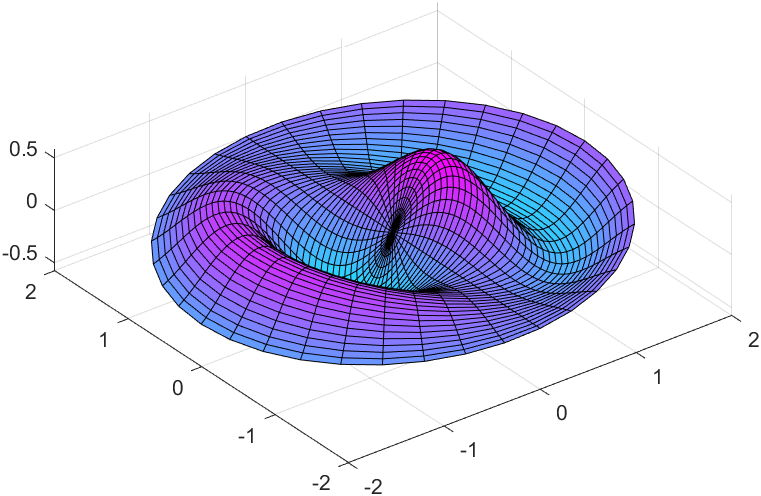
\includegraphics[width=0.27\textwidth]{1.1.png}}%
    \subfloat[\centering J1.2]{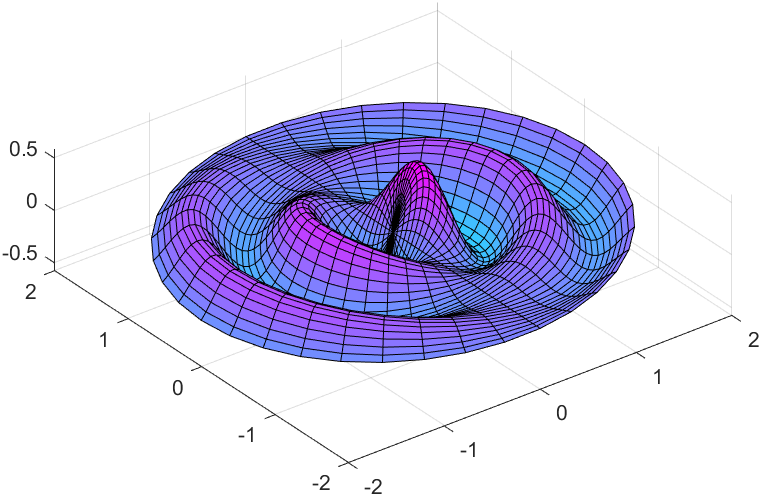
\includegraphics[width=0.27\textwidth]{1.2.png}}%
    \subfloat[\centering J1.3]{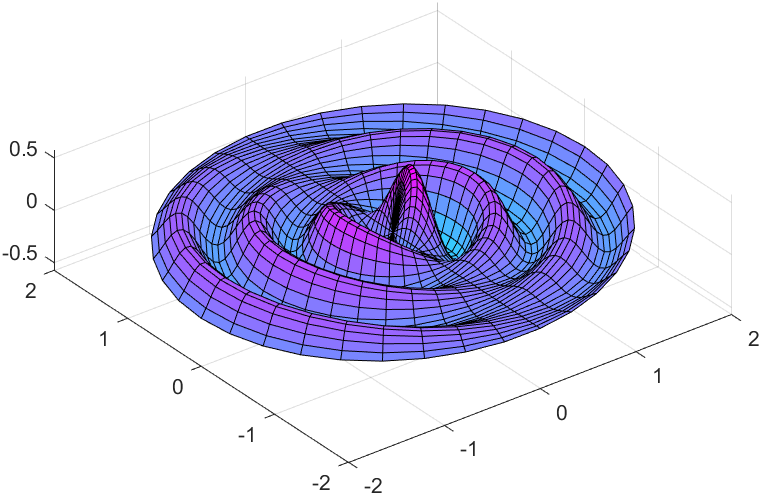
\includegraphics[width=0.27\textwidth]{1.3.png}}%
    \caption{J1.1-J1.3 @ $\lambda= 3.83,7.01, 10.17$.}
    \label{fig:J1}
\end{figure}\begin{figure}
    \centering
    \subfloat[\centering J2 .1]{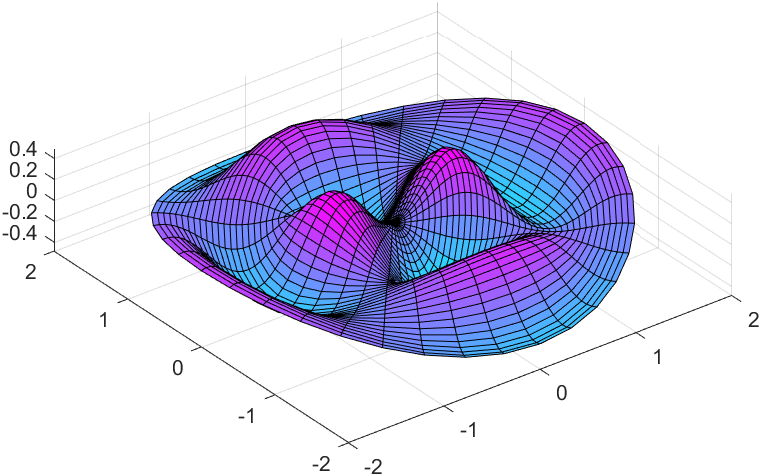
\includegraphics[width=0.27\textwidth]{2.1.png}}%
    \subfloat[\centering J2.2]{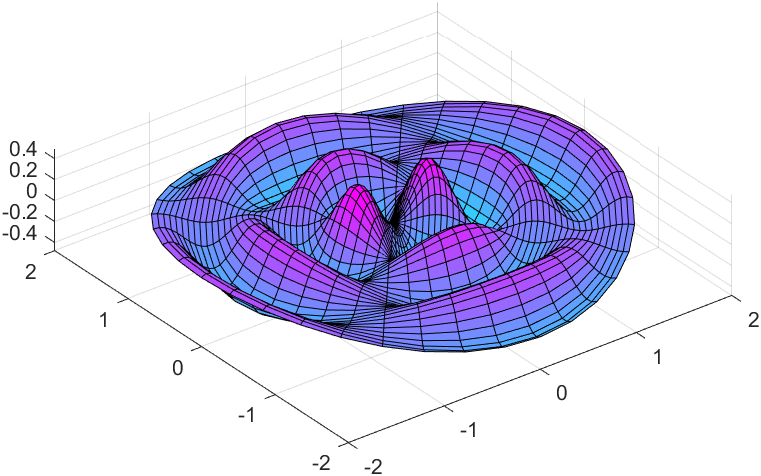
\includegraphics[width=0.27\textwidth]{2.2.png}}%
    \subfloat[\centering J2.3]{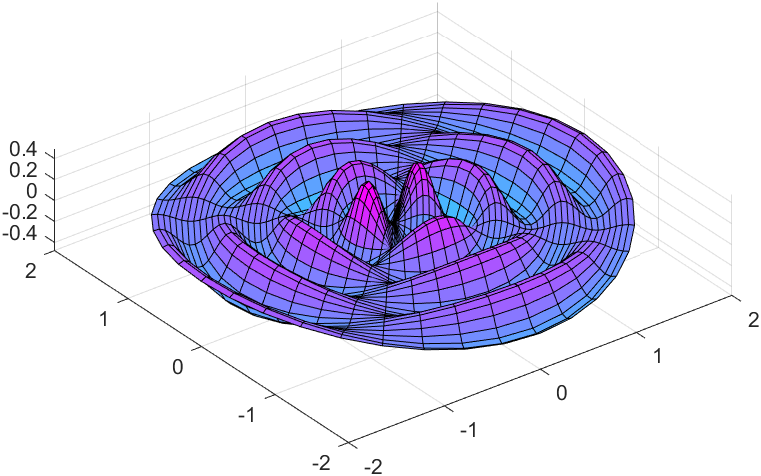
\includegraphics[width=0.27\textwidth]{2.3.png}}%
    \caption{J2.1-J2.3 @ $\lambda= 5.14,8.41, 11.62$.}
    \label{fig:J2}
\end{figure}\begin{figure}
    \centering
    \subfloat[\centering J3 .1]{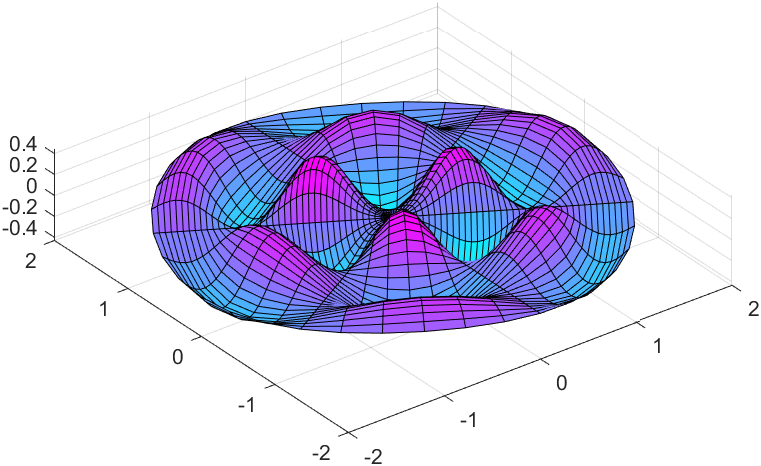
\includegraphics[width=0.27\textwidth]{3.1.png}}%
    \subfloat[\centering J3.2]{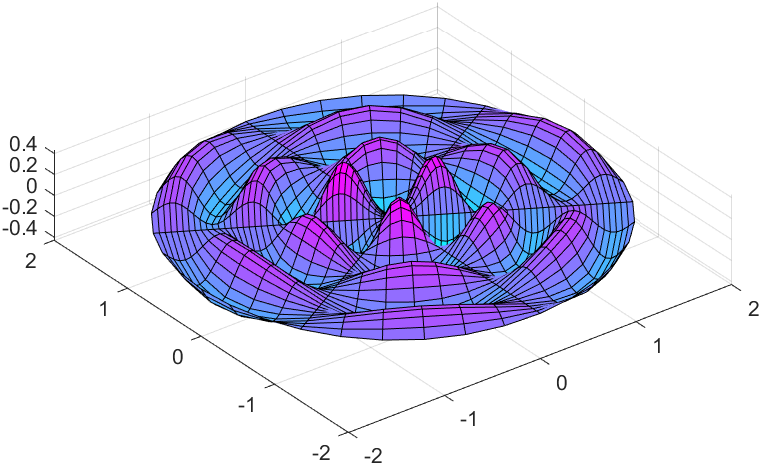
\includegraphics[width=0.27\textwidth]{3.2.png}}%
    \subfloat[\centering J3.3]{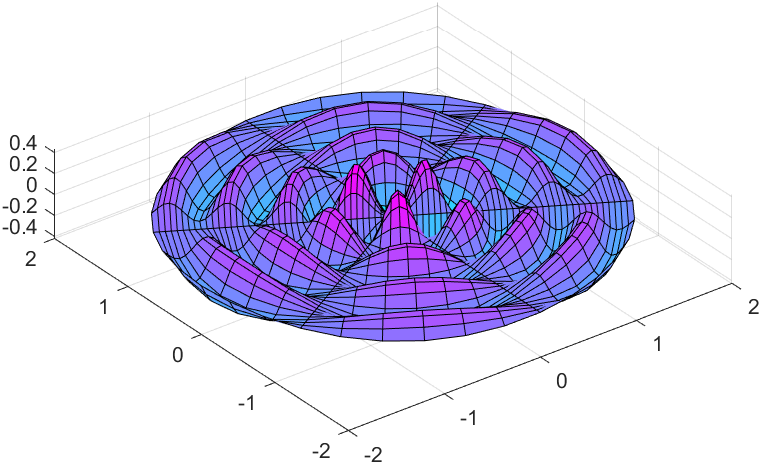
\includegraphics[width=0.27\textwidth]{3.3.png}}%
    \caption{J3.1-J3.3 @ $\lambda= 6.38,9.76, 13.01$.}
    \label{fig:J3}
\end{figure}
\clearpage
\subsubsection{Matlab Graphs}
The wave-functions resulting from the parings of n and $\lambda_{nm}$ can be calculated using Matlab and are shown below. Note: the wave functions are of the form:

\begin{equation*}
    \psi_{n,m}(r,\theta)=R_{n,m}(r)\Theta_{n}(\theta)=J_{n}(\lambda_{n,m}r)(A\cos(n\theta)+B\sin(n\theta))
\end{equation*}
For visualization purposes, the following values were set $A=1, B=0, a=1$
\begin{figure}
\centering
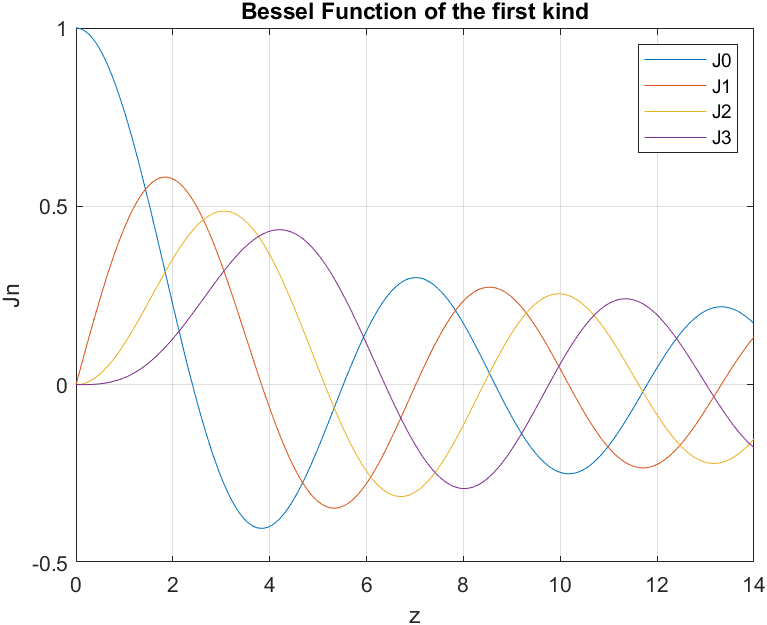
\includegraphics[width=0.75\textwidth]{Besselfotfk.png}
\end{figure}
\clearpage
\section{MATLAB Code}
\begin{lstlisting}[h]
\inputminted{matlab}{polarsurf.m}
\caption{Code adapted from Prof. Brody Johnson}
\label{listing:examplecode}
\end{lstlisting}

\begin{lstlisting}[h]
\inputminted{matlab}{polgraphs.m}
\caption{Code adapted from Prof. Brody Johnson}
\label{listing:examplecode}
\end{lstlisting}

\begin{lstlisting}[frame=sing]
\centering
\inputminted{matlab}{bessel.m}
\caption{Plots bessel functions}
\label{listing:examplecode}
\end{lstlisting}

\begin{lstlisting}[h]
\inputminted{matlab}{wavefunction.m}
\caption{Plots wave functions}
\label{listing:examplecode}
\end{lstlisting}

\clearpage
\section{References}

[1]P. Atkins and J. de Paula, Physical Chemistry, 7th ed., W.H. Freeman and Company, New York,
2002.
\newline
[2] [Prof. Brody Dylan Johnson] [Bessel's Equation and the Wave Equation on a Disk]. December 5, 2019. 
\newline
[3][Prof. Paola Cappellaro]. [Introduction To Applied Nuclear Physics]. [Spring 2012]. Massachusetts Institute of Technology: MIT OpenCouseWare, https://ocw.mit.edu/. License: Creative Commons BY-NC-SA.

\end{document}
